\subsection{Dvojitá symetrická jáma}
	\begin{figure}[!htbp]
	\centering
	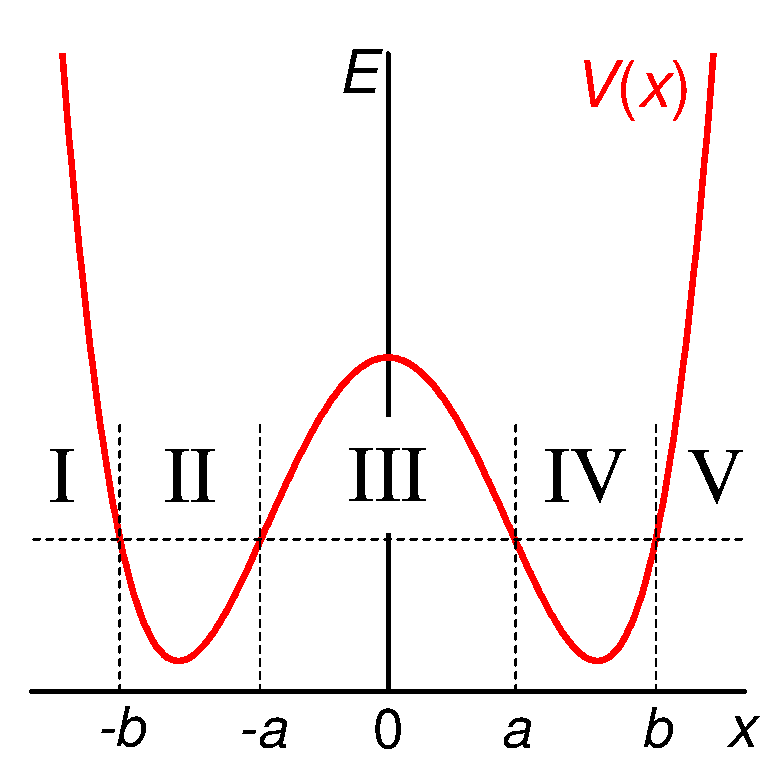
\epsfig{file=figures/dw.eps,width=0.5\linewidth,keepaspectratio}
	\caption{
		Potenciál dvojité symetrické jámy.
	}
	\label{fig:DoubleWell}
	\end{figure}	

	Částice o hmotnosti $M$ se pohybuje v sudém dvoujámovém potenciálu $V(x)=V(-x)$, viz obrázek~\ref{fig:DoubleWell}.
	Kdyby byly obě jámy oddělené nekonečně vysokou bariérou, 
	všechny energetické hladiny by byly dvakrát degenerované a odpovídající vlnové funkce by byly sudé a liché.
	Důsledkem nenulové pravděpodobnosti tunelování přes bariéru, která je v obrázku označena jako oblast III, 
	však dojde k interakci mezi hladinami a rozštěpení těchto degenerovaných dubletů.	
	\begin{enumerate}
	\item
		Nalezněte vztah pro vzdálenost $\Delta E$ mezi hladinami v dubletu pro obecný symetrický dvoujámový potenciál.
		
	\item
		Určete tuto vzdálenost pro speciální potenciál ve tvaru
		\begin{equation}
			\label{eq:DoubleWellPotential}
			V(x)=\frac{g^{2}}{8}\left(x^{2}-x_{0}^{2}\right)^{2},
		\end{equation}
		kde $x_{0}$ určuje $x$-ové souřadnice minim, $g$ je konstanta.
		Předpokládejte, že energie je dostatečně hluboko v jamách, kde lze potenciál $V(x)$ aproximovat potenciálem harmonického oscilátoru.
	
	\item
		Srovnejte číselně s výsledkem úkolu ze 3. cvičení zimního semestru.	
	\end{enumerate}

\begin{solution}
	\begin{enumerate}
	\item
		Tunelující systém se rozdělí na pět oblastí podle obrázku~\ref{fig:DoubleWell}.
		Všechny výpočty budou ve zkrácené notaci~\eqref{eq:WKBNotation}.
		Využívat se budou navazovací podmínky~\eqref{eq:WKBConnectionDown1}---\eqref{eq:WKBConnectionUp2}.
		
		\begin{itemize}
		\item
			V oblasti I musí vlnová funkce exponenciálně ubývat pro $x\rightarrow-\infty$, takže
			\begin{equation}
				\psi_{\mathrm{I}}(x)=\frac{C}{\sqrt{\abs{p(x)}}}\e^{-\frac{1}{\hbar}\int_{x}^{-b}\abs{p(x')}\d x'}=\lambda\e^{-I_{x}^{-b}}.
			\end{equation}
			
		\item
			Do oblasti II se vlnovou funkci napojí pomocí vztahů~\eqref{eq:WKBConnectionDown1}---\eqref{eq:WKBConnectionDown2}:
			\begin{equation}
				\psi_{\mathrm{II}}(x)=2\lambda\sin{\left[I_{-b}^{x}+\frac{\pi}{4}\right]}.
			\end{equation}
			Vlnovou funkci je nyní potřeba upravit do takové formy, aby bylo možné pro navázání do oblasti III použít vztahů~\eqref{eq:WKBConnectionUp1}---\eqref{eq:WKBConnectionUp2}:
			\begin{align}
				\psi_{\mathrm{II}}(x)
					&=2\lambda\underbrace{\sin{\left[I_{-b}^{-a}-I_{x}^{-a}+\frac{\pi}{4}\right]}}_{\sin{(a+b)}=\sin{a}\cos{b}+\cos{a}\sin{b}}\nonumber\\
					&=2\lambda\left\{\underbrace{\sin{I_{-b}^{-a}}}_{S}\cos\left[-I_{x}^{-a}+\frac{\pi}{4}\right]+\underbrace{\cos{I_{-b}^{-a}}}_{C}\sin\left[-\int_{x}^{-a}+\frac{\pi}{4}\right]\right\}
			\end{align}
			Je nutné ošetřit i znaménko $-$ před integrály v argumentech sinu a cosinu.
			K tomu se využijí vztahy
			\begin{align}
				\cos\left[-I+\frac{\pi}{4}\right]
					&\stackrel{\cos\text{ sudá}}{=}\cos\left[I-\frac{\pi}{4}\right]=\underbrace{\cos\left[I+\frac{\pi}{4}-\frac{\pi}{2}\right]}_{\cos{(a+b)}=\cos{a}\cos{b}-\sin{a}\sin{b}}\nonumber\\
					&=\cos\left[I+\frac{\pi}{4}\right]\underbrace{\cos\left(-\frac{\pi}{2}\right)}_{0}-\sin\left[I+\frac{\pi}{4}\right]\underbrace{\sin\left(-\frac{\pi}{2}\right)}_{-1}\nonumber\\
					&=\sin\left[I+\frac{\pi}{4}\right]\,,
			\end{align}
			a analogicky
			\begin{equation}
				\sin\left[-I+\frac{\pi}{4}\right]=\cos\left[I+\frac{\pi}{4}\right].
			\end{equation}
			Vlnovou funkci v oblasti II lze tedy zapsat ve tvaru
			\begin{equation}
				\psi_{\mathrm{II}}(x)=2\lambda\left\{S\sin\left[I_{x}^{-a}+\frac{\pi}{4}\right]+C\cos\left[I_{x}^{-a}+\frac{\pi}{4}\right]\right\}.
			\end{equation}
		
		\item
			Do oblasti III se posuneme za pomoci sešívacích vztahů~\eqref{eq:WKBConnectionUp1}---\eqref{eq:WKBConnectionUp2} a vlnovou funkci ihned upravíme pro navázání do následující oblasti IV:
			\begin{align}
				\psi_{\mathrm{III}}(x)
					&=\lambda S\e^{-I_{-a}^{x}}+2\lambda C\e^{I_{-a}^{x}}\nonumber\\
					&=\lambda S\underbrace{\e^{-I_{-a}^{a}}}_{F}\e^{I_{x}^{a}}+2\lambda C\e^{I_{-a}^{a}}\e^{-I_{x}^{a}}\nonumber\\
					&=\lambda SF\e^{I_{x}^{a}}+\frac{2\lambda C}{F}\e^{-I_{x}^{a}}
			\end{align}
			
		\item
			V navazování se pokračuje dále do oblasti IV pomocí vztahů~\eqref{eq:WKBConnectionDown1}---\eqref{eq:WKBConnectionDown2}:
			\begin{align}
				\psi_{\mathrm{IV}}(x)
					&=\lambda SF\cos\left[I_{a}^{x}+\frac{\pi}{4}\right]+\frac{4\lambda C}{F}\sin\left[I_{a}^{x}+\frac{\pi}{4}\right]\nonumber\\
					&=\lambda SF\cos\left[I_{a}^{b}-I_{x}^{b}+\frac{\pi}{4}\right]+\frac{4\lambda C}{F}\sin\left[I_{a}^{b}-I_{x}^{b}+\frac{\pi}{4}\right]\nonumber\\
					&=\lambda SF\left\{C\sin\left[I_{x}^{b}+\frac{\pi}{4}\right]-S\cos\left[I_{x}^{b}+\frac{\pi}{4}\right]\right\}\nonumber\\
					&\qquad+\frac{4\lambda C}{F}\left\{S\sin\left[I_{x}^{b}+\frac{\pi}{4}\right]+C\cos\left[I_{x}^{b}+\frac{\pi}{4}\right]\right\}\nonumber\\
					&=\lambda SC\left(F+\frac{4}{F}\right)\sin\left[I_{x}^{b}+\frac{\pi}{4}\right]+\lambda\left(-S^{2}F+\frac{4C^{2}}{F}\right)\cos\left[I_{x}^{b}+\frac{\pi}{4}\right].
			\end{align}
			Využívá se zde sudosti potenciálu, díky níž
			\begin{align}
				V(x)&=V(-x) && \Longrightarrow & p(x)&=p(-x) && \Longrightarrow & I_{-b}^{-a}&=I_{a}^{b}.
			\end{align}
			
		\item
			Poslední navazování do oblasti V se provedeme opět pomocí vztahů~\eqref{eq:WKBConnectionUp1}---\eqref{eq:WKBConnectionUp2}:
			\begin{equation}
				\psi_{\mathrm{V}}(x)=\frac{\lambda SC}{2}\left(F+\frac{4}{F}\right)\e^{-I_{b}^{x}}+\underbrace{\lambda\left(-S^{2}F+\frac{4C^{2}}{F}\right)}_{Z}\e^{I_{b}^{x}}
			\end{equation}		
		\end{itemize}
	
		Celková vlnová funkce musí být normovatelná (kvadraticky integrovatelná), tj. nesmí divergovat  pro $x\rightarrow\infty$.
		Musí být tedy splněno $Z=0$, tj.
		\begin{align}
			\lambda\left(-S^{2}F+\frac{4C^{2}}{F}\right)&=0\nonumber\\
			S^{2}&=\frac{4C^{2}}{F^{2}}\nonumber\\
			\frac{C}{S}&=\pm\frac{1}{2}F
		\end{align}
		To po dosazení za $S$, $C$ a $F$ vede na rovnici
		\begin{align}
			\cotg{\frac{1}{\hbar}\int_{a}^{b}p(x)\d x}=\pm\frac{1}{2}\e^{-\frac{1}{\hbar}\int_{-a}^{a}\abs{p(x)}\d x}.
		\end{align}
		
		Následovat bude několik aproximací. 
		Předně budeme předpokládat, že prostupnost bariéry III je malá, takže $F\approx0$ a lze psát
		\begin{equation}
			\pm\frac{1}{2}F\approx\cotg{\left[\mp\frac{1}{2}F+\pi\left(n+\frac{1}{2}\right)\right]},
		\end{equation}
		kde $n\in\mathbb{N}_{0}$.
		To vede k rovnici (kvantovací podmínce)
		\begin{equation}
			\label{eq:DoubleWellE}
			\frac{1}{\hbar}\int_{a}^{b}p(x)\d x=\pi\left(n+\frac{1}{2}\right)\pm\frac{1}{2}\e^{-\frac{1}{\hbar}\int_{-a}^{a}\abs{p(x)}\d x}
		\end{equation}
	
		Kdyby nebylo tunelování mezi dvěma jamami, spektrum $E_{n}^{(0)}$ by na základě Bohrova-Sommerfeldova kvantování~\eqref{eq:BohrSommerfeld} bylo dáno rovnicí
		\begin{equation}
			\int_{a}^{b}\sqrt{2M\left[E_{n}^{(0)}-V(x)\right]}\,\d x=\pi\hbar\left(n+\frac{1}{2}\right).
		\end{equation}
		Ve skutečnosti však dochází k tunelování a spektrum je dáno rovnicí~\eqref{eq:DoubleWellE}.
		Označme
		\begin{equation}
			E_{n}=E_{n}^{(0)}+\epsilon.
		\end{equation}
		a rozviňme levou stranu rovnice~\eqref{eq:DoubleWellE} okolo $E_{n}^{(0)}$:
		\begin{align}
			\frac{1}{\hbar}\int_{a}^{b}\underbrace{\sqrt{2M\left[E_{n}-V(x)\right]}}_{p(x;E_{n})}\,\d x
				&=\frac{1}{\hbar}\int_{a}^{b}p(x;E_{n}^{(0)})\d x+\frac{\epsilon}{\hbar}\int_{a}^{b}\partialderivative{p}{E}(x;E_{n}^{(0)})\d x+\dotsb\nonumber\\
				&\approx\pi\left(n+\frac{1}{2}\right)+\frac{\epsilon}{\hbar}\underbrace{2M\int_{a}^{b}\frac{\d x}{\sqrt{2M\left[E_{n}^{(0)}-V(x)\right]}}}_{\int_{a}^{b}\frac{\d x}{v(x)}=\frac{1}{2}\oint\frac{\d x}{v(x)}=\frac{T}{2}}\,,
		\end{align}
		kde $T$ odpovídá periodě klasické trajektorie na energii $E_{n}^{(0)}$ (úhlová frekvence je $\Omega=2\pi/T$).
		Dosazení do~\eqref{eq:DoubleWellE} vede k jednoduchému vztahu
		\begin{equation}
			\epsilon=\pm\frac{\hbar\Omega}{2\pi}E
		\end{equation}
		z něhož lze určit rozštěpení hladin jako
		\begin{equation}
			\label{eq:DoubleWellSplit}
			\important{\Delta E_{n}=\frac{\hbar\Omega}{\pi}\e^{-\frac{1}{\hbar}\int_{-a}^{a}\abs{p(x)}\d x}}.
		\end{equation}
	
	\item
		Za předpokladu, že se částice nachází na energii dostatečně blízko dnu jámy, lze potenciál~\eqref{eq:DoubleWellPotential} rozvinout okolo $x_{0}$:
		\begin{align}
			V(x)
				&=\frac{g^{2}}{8}\left(x+x_{0}\right)^{2}{\underbrace{\left(x-x_{0}\right)}_{y}}^{2}=\frac{g^{2}}{8}\left(y+2x_{0}\right)^{2}y^{2}\nonumber\\
				&\approx\frac{1}{2}g^{2}x_{0}^{2}y^{2}=\frac{1}{2}M\Omega^{2}y^{2}\,,
		\end{align}
		takže pohyb hluboko v jámě přibližně odpovídá periodickému pohybu harmonického oscilátoru s frekvencí
		\begin{equation}
			\Omega=\frac{gx_{0}}{\sqrt{M}}
		\end{equation}
		a spektrem
		\begin{equation}
			E_{n}=\hbar\Omega\left(n+\frac{1}{2}\right).
		\end{equation}
		Body obratu (řešení rovnice $V(x)=E_{n}$) pak jsou
		\begin{equation}
			\begin{array}{c}a \\ b\end{array}=x_{0}\mp\sqrt{\frac{\hbar}{M\Omega}\left(n+\frac{1}{2}\right)}
		\end{equation}
		a speciálně pro základní stav $n=0$
		\begin{subequations}	
			\begin{align}
				a&=x_{0}-\sqrt{\frac{\hbar}{M\Omega}},\\ 
				b&=x_{0}+\sqrt{\frac{\hbar}{M\Omega}}.
			\end{align}
		\end{subequations}
			
		Integrál z kvantovací podmínky~\eqref{eq:DoubleWellE} je
		\begin{align}
			\hbar I_{-a}^{a}
				&=2\hbar I_{0}^{a}=2\int_{0}^{a}\sqrt{2M\left[\frac{g^{2}}{8}\left(x_{0}^{2}-x^{2}\right)^{2}-\frac{1}{2}\hbar\Omega\right]}\,\d x\nonumber\\
				&=\int_{0}^{a}\underbrace{g}_{\frac{\Omega}{x_{0}}\sqrt{M}}\sqrt{M}\left(x_{0}^{2}-x^{2}\right)\sqrt{1-\frac{4\hbar\Omega}{g^{2}\left(x_{0}^{2}-x^{2}\right)^{2}}}\,\d x\nonumber\\
				&\approx\int_{0}^{a}\frac{M\Omega\left(x_{0}^{2}-x^{2}\right)}{x_{0}}\d x-2\int_{0}^{a}\frac{\hbar x_{0}}{x_{0}^{2}-x^{2}}\d x\nonumber\\
				&=\int_{0}^{a}\left[M\Omega x_{0}^{2}-\frac{M\Omega x^{2}}{x_{0}}-\frac{\hbar}{x_{0}-x}-\frac{\hbar}{x_{0}+x}\right]\d x\nonumber\\
				&=\left[M\Omega x_{0}^{2}x-\frac{M\Omega x^{3}}{3x_{0}}+\hbar\ln\left(x_{0}-x\right)-\hbar\ln\left(x_{0}+x\right)\right]_{0}^{a}\nonumber\\
				&=M\Omega x_{0}\left(x_{0}-\sqrt{\frac{\hbar}{M\Omega}}\right)
					-\underbrace{\frac{M\Omega}{3x_{0}}\left(x_{0}-\sqrt{\frac{\hbar}{M\Omega}}\right)^{3}}_{\approx\frac{M\Omega x_{0}^{2}}{3}\left(1-\frac{3}{x_{0}}\sqrt{\frac{\hbar}{M\Omega}}+\frac{3}{x_{0}^{2}}\frac{\hbar}{M\Omega}\right)}
					+\underbrace{\hbar\ln{\sqrt{\frac{\hbar}{M\Omega}}}}_{\hbar\ln{x_{0}}+\hbar\ln{\frac{1}{x_{0}}\sqrt{\frac{\hbar}{M\Omega}}}}\nonumber\\
				&\qquad-\underbrace{\hbar\ln{\left(2x_{0}-\sqrt{\frac{\hbar}{M\Omega}}\right)}}_{\hbar\ln{x_{0}}+\hbar\ln\left(2-\frac{1}{x_{0}}\sqrt{\frac{\hbar}{M\Omega}}\right)}\nonumber\\
				&\approx\frac{2M\Omega x_{0}^{2}}{3}-\hbar+\hbar\ln\sqrt{\frac{\hbar}{4M\Omega x_{0}^{2}}}+\mathcal{O}\left(\hbar^{\frac{2}{3}}\right),
		\end{align}
		za předpokladu, že Planckova konstanta $\hbar$ je oproti ostatním veličinám malý parametr.
		
		Po dosazení do~\eqref{eq:DoubleWellSplit} vychází pro vzdálenost hladin v dubletech
		\begin{equation}
			\Delta E_{0}
				=\frac{\Omega\hbar}{\pi}\e^{-I_{-a}^{a}}\approx\frac{\Omega\hbar}{\pi}\sqrt{\frac{4M\Omega x_{0}^{2}}{\hbar}}\e^{-\frac{2M\Omega x_{0}^{2}}{3\hbar}+1}
				=\frac{2}{\pi}\sqrt{\frac{\hbar g^{3}x_{0}^{5}}{M}}\e^{-\frac{2\sqrt{M}g x_{0}^{3}}{3\hbar}+1}.
		\end{equation}
		Sbírka~\cite{Cini2012} uvádí výsledek odlišně
		\begin{equation}
			\Delta E_{0}'=2\sqrt{\frac{\hbar g^{3}x_{0}^{5}}{M}}\e^{-\frac{2\sqrt{M}g x_{0}^{3}}{3\hbar}}\,,
		\end{equation}
		a to i přesto, že integrál $I_{-a}^{a}$ v ní vychází stejně jako zde.
		Tento výraz $\Delta E_{0}'$ nicméně lépe souhlasí s přesnějšími metodami, viz např. následující bod.
			
	\item
		Dvoujámový potenciál, se kterým budeme nyní získaný výsledek srovnávat, má tvar
		\begin{equation}
			V(x)=-\frac{1}{2}x^{2}+x^{4}=\left(x^{2}-\frac{1}{4}\right)^{2}-\frac{1}{16},
		\end{equation}
		takže se jedná přibližně o potenciál~\eqref{eq:DoubleWellPotential} s
		\begin{equation}
			g=2\sqrt{2}\,,\qquad x_{0}=\frac{1}{2}
		\end{equation}
		a spektrum je posunuté o $\frac{1}{16}$ energetické jednotky dolů.
		
		Pro dostatečně malé hodnoty $\hbar$ (v úloze se počítalo s $\hbar=0.02$) dostaneme pro základní stav
		\begin{align}
			\Omega&=\frac{g x_{0}}{\sqrt{M}}=\sqrt{2}\approx1.4142\nonumber\\
			E_{0}&=\frac{1}{2}\hbar\Omega-\frac{1}{16}\approx-0.0484\nonumber\\
			\Delta E_{0}'&=1.81\cdot 10^{-6}
		\end{align}
		Naproti tomu na základě numerické diagonalizace jsme dostali
		\begin{align}
			E_{0}&=-0.0489 & \Delta E=1.86\cdot 10^{-6}.
		\end{align}
		Pro menší hodnoty $\hbar$ bychom dostali lepší shodu.						
	\end{enumerate}
\end{solution}
	
